\documentclass[11pt]{article}
\usepackage[letterpaper,margin=0.72in,headheight=15pt]{geometry}
\usepackage{amsmath,booktabs,enumitem,fancyhdr,graphicx,listings,microtype,tabularx,xcolor}
\usepackage[hidelinks]{hyperref}
\graphicspath{{docs/lessons/assets/}{../assets/}}
\definecolor{codebg}{gray}{0.97}
\pagestyle{fancy}\fancyhf{}\lhead{\textsc{ADK lesson 022}}
\rhead{The memory trail}\cfoot{\thepage}
\setlength{\parindent}{0pt}\setlength{\parskip}{5pt}
\setlist{nosep,leftmargin=1.45em}
\renewcommand{\arraystretch}{1.16}
\lstdefinestyle{adkcpp}{language=C++,basicstyle=\ttfamily\small,
backgroundcolor=\color{codebg},frame=single,columns=fullflexible,
keepspaces=true,showstringspaces=false,breaklines=true}
\hypersetup{
pdftitle={ADK Lesson 022: The Memory Trail},
pdfauthor={Kevin Shanahan},
pdfsubject={A fast visible adventure through analog samples and deterministic records},
pdflang={en-US}}
\begin{document}

\begin{center}
{\Huge\bfseries The memory trail}\\[4pt]
{\Large Lesson 022 --- turn a knob, leave a visible record}\\[6pt]
\textit{Each successful software step earns a pulse you can see.}
\end{center}

\begin{tabularx}{\linewidth}{@{}>{\bfseries}lX>{\bfseries}lX@{}}
Time & about 45 minutes & Board & Arduino Mega 2560\\
Prerequisites & Lessons 001--021 & Kind & component\\
Payoffs & live pulse length, eighth-record flourish & Energy & E1, USB only\\
Physical parts & potentiometer, LED, 1 k\(\Omega\) resistor & Storage & model only\\
\end{tabularx}

This lesson is a small record-making machine. Turn a 10 k\(\Omega\)
potentiometer. The Mega samples A0, combines that value with a simulated clock,
runs the bytes through recording-only I2C and SPI software, synchronizes a
fixed in-memory model, then lights D13. A drier setting makes a short pulse; a
wetter setting makes a longer one. Every eighth record earns an unmistakable
1.2-second pulse.

\textbf{Honest boundary.} There is no RTC module, storage card, soil probe, or
physical I2C/SPI peripheral in this build. The authorized Elegoo set contains
no removable-storage specimen. D20, D21, D49, D50, D51, and D52 remain empty.
The sketch generates no bus waveform and proves no physical clock or durable
media behavior. A future RTC stage requires the exact module revision,
markings, voltage, address, primary datasheet, and electrical review first.

\textbf{Stop rule.} Unplug USB before moving wires. Stop for heat, smell,
smoke, repeated USB resets, or any disagreement between the drawing and the
part in hand.

\section*{Adventure}

Build the input first and use its pulse length as evidence. Count eight
records to earn the software-restart reward, then keep watching for the fixed
safe ending. Each payoff depends on the one before it.

Use the canonical \texttt{Lesson022OwnedBuses} sketch throughout. It has a
fixed two-minute deadline. At that deadline both indicators go dark, stay
inactive for 250 ms, release their resources, and wait for Reset. Turning the
knob cannot postpone the ending.

\section*{Stage 1: wire one literal circuit}

Gather a Mega 2560, USB cable, breadboard, 10 k\(\Omega\) linear
potentiometer, ordinary LED, 1 k\(\Omega\) resistor, and jumpers. The built-in
D13 LED is the activity light; do not build another D13 branch.

\begin{center}
% ADK visual: pencil
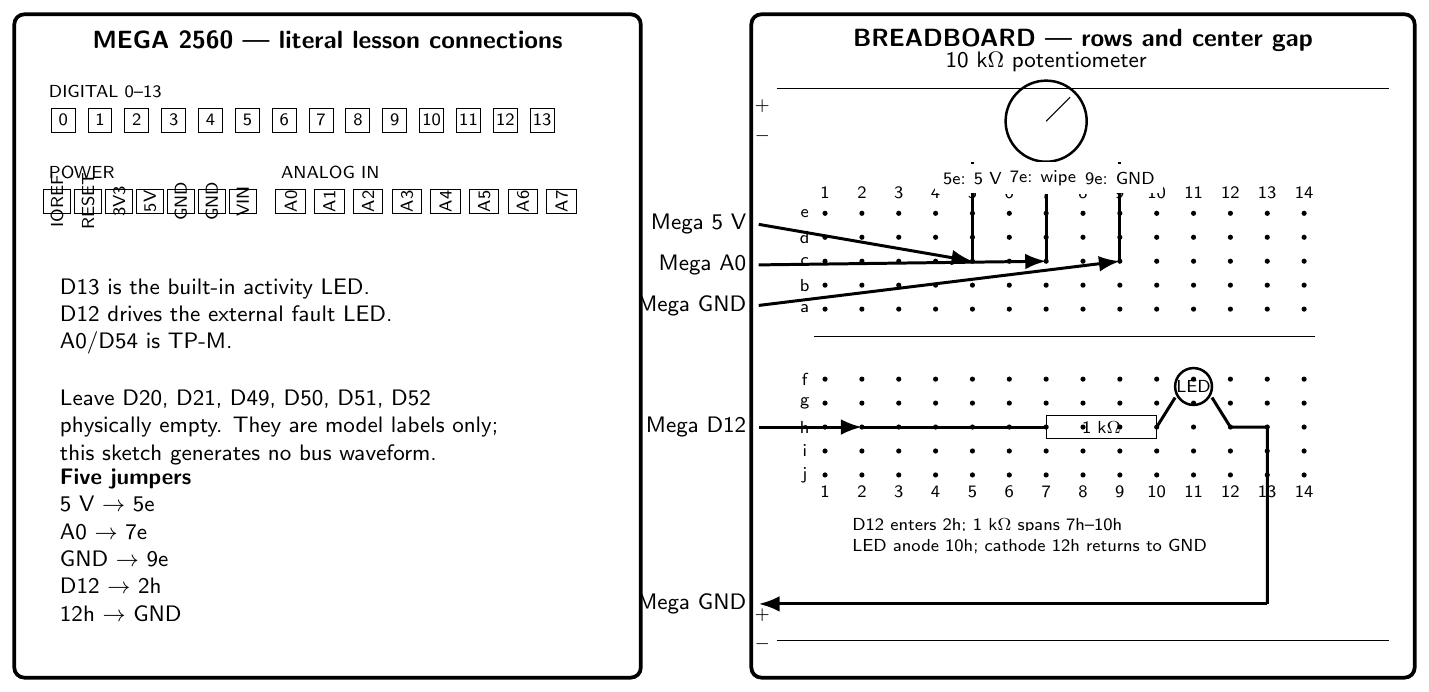
\includegraphics[width=\linewidth,height=0.48\textheight,keepaspectratio]
{022-owned-buses-pencil.png}
\end{center}
\textbf{Plate 1: actual headers and breadboard paths.} The potentiometer's two
outer legs go to 5 V and GND; its center wiper goes to A0. D12 goes through
the 1 k\(\Omega\) resistor to the external LED anode; the cathode returns to
the same GND. Verify the potentiometer's center wiper from its own drawing or
with a meter before power.

\begin{tabularx}{\linewidth}{@{}l l X@{}}
\toprule
Name & Mega pin & Exact path\\\midrule
TP-M & A0 / D54 & potentiometer center wiper\\
Pot rails & 5 V, GND & one outer leg to each rail\\
Activity & D13 & built-in LED only\\
Fault & D12 & D12 \(\rightarrow\) 1 k\(\Omega\) \(\rightarrow\) LED anode;
cathode \(\rightarrow\) GND\\
Model labels & D20/D21, D49--D52 & leave every pin physically empty\\
\bottomrule
\end{tabularx}

Restore USB and upload. After the first 1.5 seconds, D13 should pulse. D12
stays dark. If D12 lights, unplug and inspect only the four physical paths in
Plate 1. Adding an RTC or card cannot repair this circuit and is not allowed.

\section*{Stage 2: play the pulse instrument}

The lesson calibration uses raw ADC counts 200 and 800 as its two chosen
endpoints. Counts between them map to 0--1000 permille. This number is a
repeatable teaching scale, not soil moisture.

\begin{tabularx}{\linewidth}{@{}c c c@{}}
\toprule
Approximate raw count & Model value & D13 reward\\\midrule
200 & 0 permille & about 0.1 s\\
500 & 500 permille & about 0.5 s\\
800 & 1000 permille & about 0.9 s\\
\bottomrule
\end{tabularx}

Turn the shaft slowly from one side to the other. The changing pulse length is
the feedback: A0 must be connected, the sample must be valid, the simulated
clock state must be valid, both recording transactions must complete, and
\texttt{sync()} must succeed before D13 turns on.

If the pulse never changes, unplug and check the center wiper at A0 and both
outer legs. If it changes backward from your preferred story, swap only the
two outer potentiometer legs. Never move the center wiper.

\section*{Stage 3: follow one record}

\begin{center}
% ADK visual: pencil
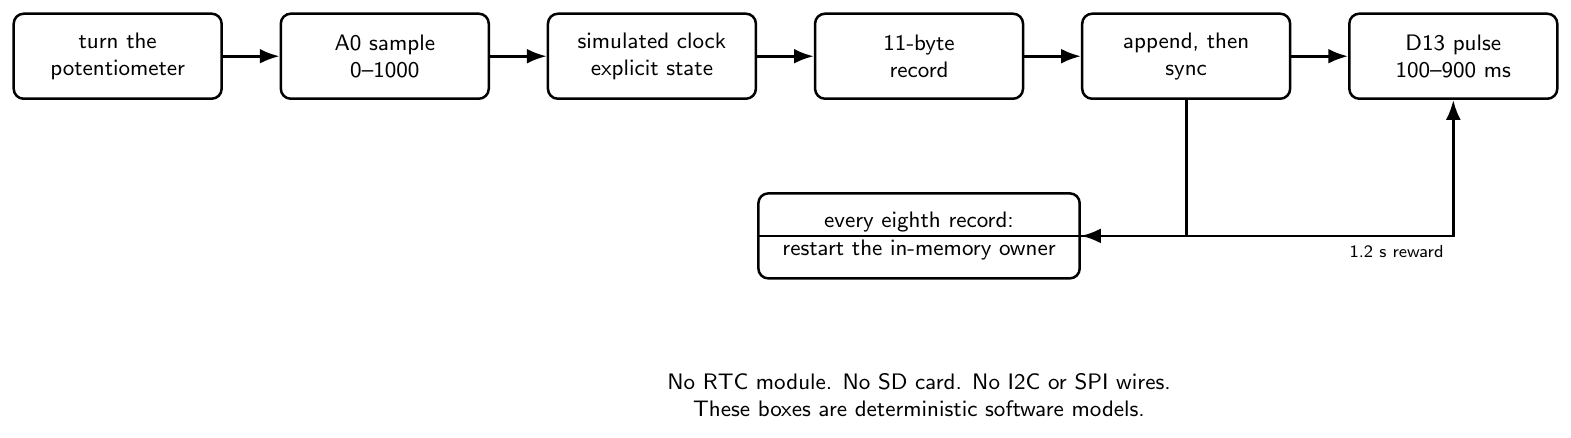
\includegraphics[width=\linewidth]{022-record-journey-pencil.png}
\end{center}
\textbf{Plate 2: the software journey.} It deliberately depicts no RTC board,
SD card, or bus wires because none exists in this lesson.

The simulated clock begins at a fixed Unix-seconds value. The 11-byte record
contains four clock bytes, one explicit clock-state byte, two raw ADC bytes,
two lesson-scale bytes, one sample-state byte, and one synthetic metadata
byte. \texttt{append()} stages the bytes. Only \texttt{sync()} advances the
model's committed prefix.

Count the ordinary pulses. The eighth is replaced by a 1.2-second flourish.
Before that flourish, the sketch shuts down and reinitializes its
\texttt{FixedStorage} owner and confirms that its committed byte count is
unchanged. That is a software-session restart inside one running sketch. It
does not survive Reset or unplugging and must never be described as SD-card or
power-loss evidence.

\section*{Stage 4: discover the ending}

Keep turning the knob if you like. Exactly two minutes after startup, D13 and
D12 become inactive. They remain inactive for a quarter second; then the
lesson releases its resources and waits. Press Reset to start a new run.

This ending is independent of input. A stuck potentiometer, rapid turning, or
the eighth-record reward cannot extend it. The visible result therefore
depends on the same lifetime policy exercised by the automated tests behind
the scenes.

\section*{What the lights actually mean}

\begin{tabularx}{\linewidth}{@{}p{0.25\linewidth}X@{}}
\toprule
What you see & What it supports\\\midrule
changing D13 pulses & A0 sampling plus the complete deterministic model path\\
1.2-second eighth pulse & in-memory owner restart preserved the committed size\\
D12 latched on & a software status failed; power down and inspect the base circuit\\
both dark at two minutes & fixed inactive hold and shutdown began\\
\bottomrule
\end{tabularx}

None of those observations supports an I2C acknowledgement, SPI clock edge,
RTC oscillator state, SD-card write, media durability, or power-loss
retention. Those claims require exact authorized hardware and measurements
that this lesson does not contain.

\section*{Under the hood}

Construction is inert. \texttt{initialize()} claims each owner before use,
and failure rolls earlier claims back. Every transfer has a bounded timeout.
The caller owns each buffer for the whole synchronous call. Shutdown is
idempotent and releases owners in reverse order.

\begin{lstlisting}[style=adkcpp]
if (observeControl (now, sample) &&
    persistRecord (now, sample))
{
    acknowledgeRecord (now, sample);
}
\end{lstlisting}

The reused library value types retain their historical
\texttt{MoistureSample} names, but this lesson uses them only as a bounded
analog calibration model. Its learner-facing input, scale, and record
vocabulary is deliberately neutral; no soil or moisture observation occurs.

The host suite retains the exhaustive work: invalid addresses and lengths,
claim conflicts, injected configure and transfer failures, chip-select
restoration, partial append at every byte, failed sync, exact restart
recovery, capacity exhaustion, every clock state, repeated shutdown,
destruction, and deterministic replay. Those checks protect the implementation
without interrupting the visible adventure.

\section*{Make it yours}

Try one change at a time: make the ordinary interval one second, change the
eighth-record flourish to a two-pulse rhythm, reverse the chosen dry/wet
endpoints in software, or draw a paper ``memory trail'' beside the LEDs.
Keep all changes inside this USB-powered, resistor-limited circuit.

\vfill\small
\textbf{Companion material.} The HTML page carries searchable pin and model
tables plus source links. This printable lesson carries the literal wiring
plates, staged visible adventure, and honest model-only hardware boundary.
\end{document}
